\documentclass[arhiv]{../izpit}
%\usepackage{fouriernc}
%\usepackage{xcolor}
%\usepackage{tikz}
\usepackage{fancyvrb}
\usepackage{enumitem}
\usepackage{tikz}
\VerbatimFootnotes{}

\begin{document}

\izpit{Programiranje I: 2.\ izpit}{9.\ februar 2021}{
  Čas reševanja je 120 minut.
  Veliko uspeha!
}

%%%%%%%%%%%%%%%%%%%%%%%%%%%%%%%%%%%%%%%%%%%%%%%%%%%%%%%%%%%%%%%%%%%%%%%
\naloga[\tocke{30}]

\podnaloga[\tocke{4}]
Napišite funkcijo, ki za trojico celih števil preveri, ali tvorijo \emph{pitagorejsko trojico}. Trojica $(a, b, c)$ je pitagorejska, če je $a^2 + b^2$ enako $c^2$.
{\small\begin{verbatim}
    pitagorejska_trojica : int * int * int -> bool

    # pitagorejska_trojica (3, 4, 5);;
    - : bool = true
    # pitagorejska_trojica (5, 4, 3);;
    - : bool = false
\end{verbatim}}

\podnaloga[\tocke{5}]
Napišite funkcijo, ki za celo število $x$ vrne celo število $a$, kjer velja $\sqrt{x} \in [a, a+1)$.
{\small\begin{verbatim}
    priblizek_korena : int -> int

    # priblizek_korena 9;;
    - : int = 3
    # priblizek_korena 17;;
    - : int = 4
\end{verbatim}}

\podnaloga[\tocke{7}]
Definirajte funkcijo, ki sprejme seznam celih števil in najprej \textbf{izpiše} vsa soda števila v seznamu, nato pa \textbf{izpiše} še vsa liha števila v seznamu. Števila naj bodo izpisana v isti vrstici in med njimi ne želimo presledkov.
{\small\begin{verbatim}
    izpisi_soda_liha : int list -> unit

    # izpisi_soda_liha [3; 1; 4; 1; 5; 9; 2];;
    4231159- : unit = ()
    # izpisi_soda_liha [2; 7; 1; 8; 2; 8; 1];;
    2828711- : unit = ()

\end{verbatim}}

\podnaloga[\tocke{7}]
Napišite funkcijo, ki sprejme seznam elementov tipa \verb|option| in preveri, da si v seznamu izmenično sledijo konstruktorji \verb|None| in 
\verb|Some|.
{\small\begin{verbatim}
    alternirajoci_konstruktorji : 'a option list -> bool

    # alternirajoci_konstruktorji [None; Some 1; None; Some 100; None];;
    - : bool = true
    # alternirajoci_konstruktorji [None; Some 1; Some 10];;
    - : bool = false
    # alternirajoci_konstruktorji [Some 1; None; Some 10; None];;
    - : bool = true
\end{verbatim}}

\podnaloga[\tocke{7}]
Funkcija \verb|najmanjsi_rezultat| naj za element \verb|x| in seznam funkcij \verb|fs| vrne \textbf{indeks} funkcije, ki ima pri argumentu \verb|x| najmanjšo vrednost izmed vseh funkcij v seznamu \verb|fs|. Ker je seznam morda prazen, naj bo rezultat tipa \verb|option|.

\textbf{Za vse točke naj bo funkcija repno rekurzivna.}

{\small\begin{verbatim}
    najmanjsi_rezultat : 'a -> ('a -> 'b) list -> int option

    # najmanjsi_rezultat (-10) [(fun x -> 10 * x); succ; (fun y -> -10 * y)];;  
    - : int option = Some 0
    # najmanjsi_rezultat 10 [(fun x -> 10 * x); succ; (fun y -> -10 * y)];;    
    - : int option = Some 2
    # najmanjsi_rezultat 30 [];;
    - : int option = None
\end{verbatim}}

%%%%%%%%%%%%%%%%%%%%%%%%%%%%%%%%%%%%%%%%%%%%%%%%%%%%%%%%%%%%%%%%%%%%%%%

\naloga[\tocke{30}]

Za učinkovitejše iskanje po leksikografsko urejenih parih bomo uporabili \emph{leksikografska drevesa}, ki jih ustvarimo s pomočjo binarnih dreves.

\begin{verbatim}
    type 'a tree = Empty | Node of 'a tree * 'a * 'a tree
\end{verbatim}

Leksikografsko drevo za pare tipa \verb|'a * 'b| je binarno drevo, ki ima v
vozlišču element tipa \verb|'a| (da lahko primerjamo po prvi komponenti) in pa drevo tipa \verb|'b tree| (za primerjanje po drugi komponenti).

\begin{verbatim}
    type ('a, 'b) lexi_tree = ('a * 'b tree) tree
\end{verbatim}

Par \verb|(a, b)| se nahaja v leksikografskem drevesu, če imamo v drevesu vozlišče s parom \verb|(a, subtree)| in se \verb|b| nahaja v \verb|subtree|.

Primer drevesa za pare \verb|(3, "g")|, \verb|(3, "t")|, \verb|(7, "a")|, \verb|(10, "e")|, \verb|(10, "r")|, \verb|(10, "t")| in \verb|(10, "z")| je:

\[
  \begin{tikzpicture}[level distance=2.5cm,
    level 1/.style={sibling distance=4cm},
    level 2/.style={sibling distance=2cm}
    ]
    \node[rectangle, draw, label=left:\textbf{7}] 
        {\begin{tikzpicture}[level distance=1cm]
            \node [circle,draw] {a};
        \end{tikzpicture}}
    child {node [rectangle, draw, label=left:\textbf{3}] 
        {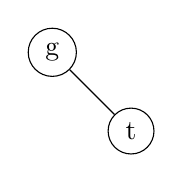
\begin{tikzpicture}[level distance=1cm, level 1/.style={sibling distance=1cm}]
            \node [circle,draw] {g}
                child { node [circle,draw, xshift=1cm] {t}};
        \end{tikzpicture}}
        }
    child {node [rectangle, draw, label=left:\textbf{10}] 
        {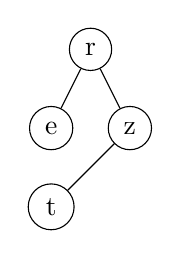
\begin{tikzpicture}[level distance=1cm, level 1/.style={sibling distance=1cm}]
            \node [circle,draw] {r}
                child { node [circle,draw] {e}}
                child { node [circle,draw] {z}
                    child {node [circle,draw, xshift=-1cm] {t}}};
        \end{tikzpicture}}
        }
    ;
  \end{tikzpicture}
\]


\podnaloga[\tocke{3}]
V OCamlu definirajte primer, ki ustreza zgornjemu leksikografskemu drevesu.

\podnaloga[\tocke{7}]
Napišite funkcijo, ki preveri ali je par prisoten v leksikografskem drevesu.

\podnaloga[\tocke{7}]
Napišite funkcijo za vstavljanje elementov v leksikografsko drevo. Če je element že v drevesu vrnite nespremenjeno drevo.

\podnaloga[\tocke{7}]
Napišite funkcijo \verb|lexi_fold|, ki sprejme funkcijo \verb|f| in začetno vrednost akumulatorja, nato pa funkcijo \verb|f| zloži preko leksikografskega drevesa. Vrstni red zlaganja je določen z leksikografsko urejenostjo.

\begin{verbatim}
    lexi_fold : ('a -> 'b -> 'c -> 'a) -> 'a -> ('b, 'c) lexi_tree -> 'a
\end{verbatim}

\podnaloga[\tocke{6}]
Definirajte funkcijo, ki vrne urejen seznam vseh elementov, ki se nahajajo v leksikografskem drevesu.


%%%%%%%%%%%%%%%%%%%%%%%%%%%%%%%%%%%%%%%%%%%%%%%%%%%%%%%%%%%%%%%%%%%%%%%

\naloga[\tocke{20}]
\emph{Nalogo lahko rešujete v Pythonu ali OCamlu.}

Psička Nara po njivi preganja krokarje. Opazila je, da jo lastnik čaka na drugem koncu polja, zato hiti k njemu, pri tem pa hoče prestrašiti kar se da veliko ubogih ptičev.

Njivo predstavimo kot matriko, ki v vsakem polju vsebuje število krokarjev, ki jih pasja navihanka prežene, če teče preko tega polja.

\[
\begin{bmatrix}
2& 3& 0& 2& 9\\
8& 3& 5& 1& 2\\
1& 2& 7& 2& 0\\
4& 3& 6& 5& 5
\end{bmatrix}
\]

\podnaloga[\tocke{10}]
Nara se nahaja v zgornjem levem kotu njive (polje $(0, 0)$). Ker se ji mudi k lastniku, se vztrajno premika desno. Na vsakem koraku se lahko premakne:
\begin{itemize}
\item desno
\item diagonalno desno-gor
\item diagonalno desno-dol
\end{itemize}

Pregon krokarjev zaključi na poljubnem skrajno desnem polju njive. Napišite funkcijo, ki izračuna največje število krokarjev, ki jih lahko nagajivka prežene.

\podnaloga[\tocke{10}]
Funkcijo iz točke (a) prilagodite tako, da ji dodatno podate indeks vrstice, v kateri Nara začne, in indeks vrstice, v kateri Nara konča. Funkcija naj vrne seznam \textbf{vseh} optimalnih poti, kjer pot predstavimo s seznamom indeksov polj, preko katerih Nara teče.
\end{document}